% Author: Izaak Neutelings (March 2019)
\documentclass[border=3pt,tikz]{standalone}
\usetikzlibrary{calc}
\tikzset{>=latex} % for LaTeX arrow head

\colorlet{knob}{blue!20!black!40}
\colorlet{mylightblue}{blue!10}
\colorlet{mydarkblue}{blue!30!black}
\tikzstyle{arrow}=[->,very thick,mydarkblue]
\tikzstyle{vector}=[->,line width=2,green!50!black]

% ANGLE
\newcommand{\getangle}[3]{%
    \pgfmathanglebetweenpoints{\pgfpointanchor{#2}{center}}
                              {\pgfpointanchor{#3}{center}}
    \global\let#1\pgfmathresult  
}


% ENGINE
\def\gas{blue!10}
\def\engine#1{
  \def\R{2}
  \def\l{1}
  \def\L{4.6}
  \def\p{1.8}
  \def\P{3.2}
  \def\Ra{.35} % crankshaft
  \def\Rb{.6}  % crankshaft
  \def\Rc{.2}  % crankshaft
  \def\a{40} % wall
  \def\b{30} % rod
  \coordinate (O)   at (0,0);
  \coordinate (CS)  at (#1:\l);
  \coordinate (P)   at (0,{\l*sin(#1)+sqrt(\P^2-(\l*cos(#1))^2)});
  \coordinate (RL)  at (180-\a:\R);
  \coordinate (RR)  at (\a:\R);
  \coordinate (TL)  at ($(RL)+(0,\L)$);
  \coordinate (TR)  at ($(RR)+(0,\L)$);
  \coordinate (T)   at ($(TL)!.5!(TR)$);
  \coordinate (PL)  at ($(RL)+(0,{\l*(1.4+sin(#1))})$);
  
  \coordinate (PR)  at ($(PL-|RR)+(0,\p)$);
  \coordinate (S)   at ($(T)+(0,.8)$);
  \coordinate (VLo) at ($(TL)!.2!(S)$);
  \coordinate (VL)  at ($(TL)!.4!(S)$);
  \coordinate (VLm) at ($(TL)!.6!(S)$);
  \coordinate (VRo) at ($(TR)!.2!(S)$);
  \coordinate (VR)  at ($(TR)!.4!(S)$);
  \coordinate (VRm) at ($(TR)!.6!(S)$);
  \getangle{\c}{CS}{P}
  \getangle{\vl}{VLo}{VLm}
  \getangle{\vr}{VRo}{VRm}
  
  % GAS
  \fill[\gas,draw=white,line width=3] (PL) -| (TR) -- (S) -- (TL) -- cycle;
  
  % CRANKSHAFT
  \draw[thick,mydarkblue,top color=blue!30!black!40,bottom color=blue!30!black!10,shading angle=180]
    (O) ++ (180+#1:\Ra) to[out={-90+#1},in={180+#1},looseness=.8]
    ($(CS)+(-90+#1:\Rb)$) arc (-90+#1:90+#1:\Rb) to[out=180+#1,in=90+#1,looseness=.8] cycle;
  
  % ROD
  \draw[thick,mydarkblue,top color=blue!30!black!50,bottom color=blue!30!black!20,shading angle=\c]
    (CS) ++ (\c-\b:\Rb) arc (\c-\b:-360+\c+\b:\Rb) -- ($(P)+(\c+90:\Rc)$) -- ($(P)+(\c-90:\Rc)$) -- cycle;
  
  % PISTON
  \draw[mydarkblue,thick,top color=blue!20!black!30,bottom color=blue!20!black!30,middle color=blue!5,shading angle=90]
    (PL) rectangle (PR);
  \draw[thick,mydarkblue,fill=knob]
    (PL) ++ (0,.65*\p) rectangle ($(PR)+(0,-.25*\p)$);
  
  % DECORATION
  \draw[thick,mydarkblue,fill=knob] (O) circle (\Rc/2);
  \draw[thick,mydarkblue,fill=knob] (CS) circle (\Rc);
  \draw[thick,mydarkblue,fill=knob] (P) circle (\Rc);
  
  % WALL
  \wall
}

% WALL
\def\wall{
  \draw[line width=4,blue!10!black!50]
    (VRo) ++ (1.5,0.6) to[out=180,in=60] (VRo) -- (TR) -- %to[out=-30,in=90,looseness=0.5]
    (RR) arc (\a:-180-\a:\R) --
    (TL) -- (VLo) to[out=110,in=0] ++ (-1.5,0.6); %to[out=90,in=200,looseness=0.8]
  \draw[line width=4,blue!10!black!50]
    (VLo) ++ (-1.5,1.3) to[out=0,in=110] (VLm) -- (S) --
    (VRm) to[out=60,in=180] ($(VRo)+(1.5,1.3)$);
    
  \fill[blue!30!black!60]
    (S) ++ (.07,.2) to[out=90,in=-150]++ (1,1.4) -- ($(S)+(1,1.74)$)
    to[out=-150,in=90] ($(S)+(-.07,.2)$);
  \draw[blue!30!black!80]
    (S) ++ (.07,.2) to[out=90,in=-150]++ (1,1.4)
    (S) ++ (-.07,.2) to[out=90,in=-150]++ (1.07,1.54);
  \draw[blue!10!black,fill=blue!20!black]
    (S) ++ (-.09,-.16) --++ (.09,-.1) coordinate (X) --++ (.09,.1) -- cycle;
  \draw[blue!30!black,fill=blue!30!black!80]
    (S) ++ (-.1,-.15) --++ (.2,0) --++ (0,.35) --++ (-.2,0) -- cycle;
}

% VALVE
\def\valveL#1{
  \fill[thick,blue!20!black]
    (VLo) ++ (\vl-90:#1) -- ($(VLm)+(\vl-90:#1)$) -- ($(VLo)!.64!(VLm)+(\vl+90:.2-#1)$) --++ (\vl+90:2)
    -- ($(VLo)!.36!(VLm)+(\vl+90:2.2-#1)$) -- ($(VLo)!.36!(VLm)+(\vl+90:.2-#1)$) -- cycle;
}

% VALVE
\def\valveR#1{
  \fill[thick,blue!20!black]
    (VRo) ++ (\vr+90:#1) -- ($(VRm)+(\vr+90:#1)$) -- ($(VRo)!.64!(VRm)+(\vr-90:.2-#1)$) --++ (\vr-90:2)
    -- ($(VRo)!.36!(VRm)+(\vr-90:2.2-#1)$) -- ($(VRo)!.36!(VRm)+(\vr-90:.2-#1)$) -- cycle;
}



\begin{document}


% INTAKE STROKE
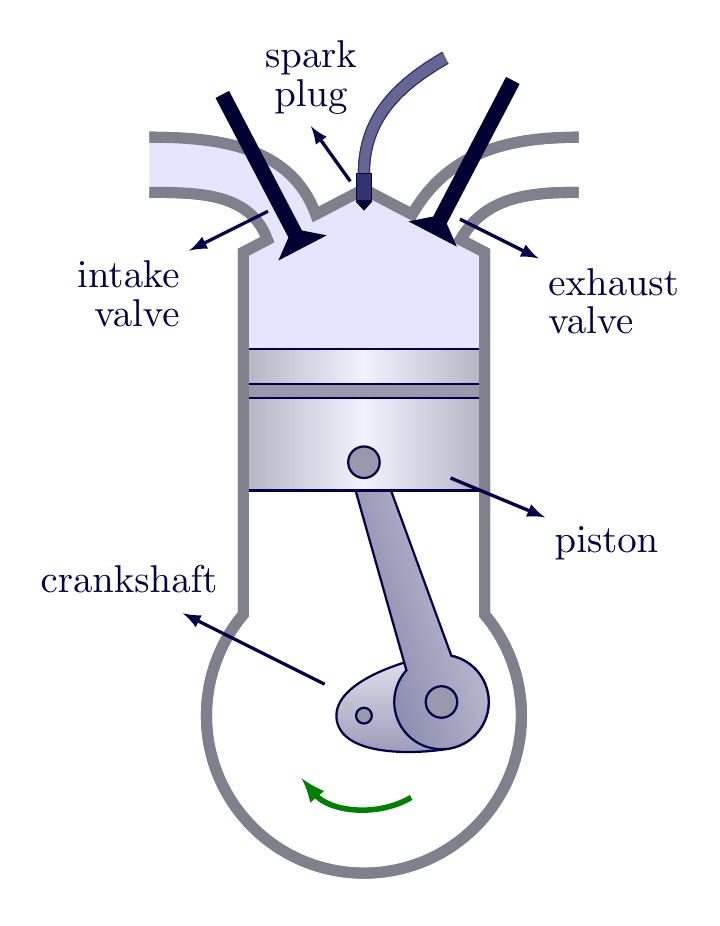
\begin{tikzpicture}
  \def\d{-60}
  \engine{10};
  \draw[vector] (\d:.6*\R) arc (\d:\d-80:.55*\R);
  \fill[\gas]
    (VLo) to[out=110,in=0] ++ (-1.5,0.6) -- ($(VLo)+(-1.5,1.3)$) to[out=0,in=110] (VLm) to[out=\vl-90,in=\vl-90] cycle;
  \wall
  \valveL{.3}
  \valveR{.1}
  
  \draw[arrow] (VL) ++ (-.3,.2) --++ (-1,-.5)
    node[below left=-2,align=right,scale=1.4] {intake\\[-2pt]valve};
  \draw[arrow] (VR) ++ (.3,.1) --++ (1,-.5)
    node[below right=-2,align=left,scale=1.4] {exhaust\\[-2pt]valve};
  \draw[arrow] (O) ++ (-.5,.4) --++ (-1.8,.9)
    node[left=-20,above left=2,scale=1.4] {crankshaft};
  \draw[arrow] (P) ++ (1.1,-.2) --++ (1.2,-.5)
    node[below right=-2,scale=1.4] {piston};
  \draw[arrow] (S) ++ (150:.2) --++ (-.5,.7)
    node[above=-1,align=center,scale=1.4] {spark\\[-2pt]plug};
  
\end{tikzpicture}


% COMPRESSION STROKE
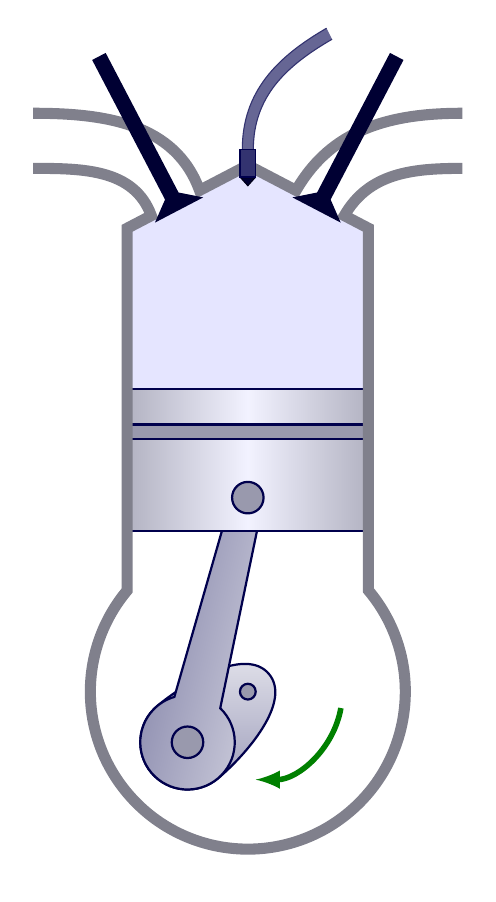
\begin{tikzpicture}
  \def\d{-10}
  \engine{-140};
  \draw[vector] (\d:.6*\R) arc (\d:\d-80:.55*\R);
  \valveL{.1}
  \valveR{.1}
\end{tikzpicture}


% IGNITION
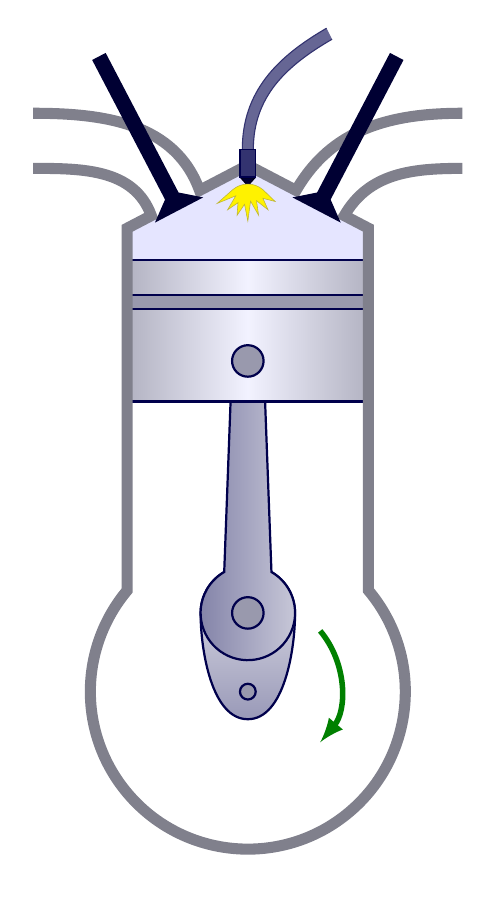
\begin{tikzpicture}
  \def\d{40}
  \engine{90};
  \draw[vector] (\d:.6*\R) arc (\d:\d-80:.55*\R);
  \valveL{.1}
  \valveR{.1}
  \draw[very thin,yellow!70!black,fill=yellow,shift={(X)}]
    ( -15:.20) -- ( -30:.40) -- ( -40:.25) -- ( -50:.40) --
    ( -60:.22) -- ( -70:.40) -- ( -80:.20) -- ( -90:.45) --
    (-100:.24) -- (-110:.40) -- (-120:.25) -- (-130:.40) --
    (-140:.20) -- (-150:.45) -- (-165:.20) to[out=40,in=140] cycle;
\end{tikzpicture}


% POWER STROKE
\def\gas{red!10}
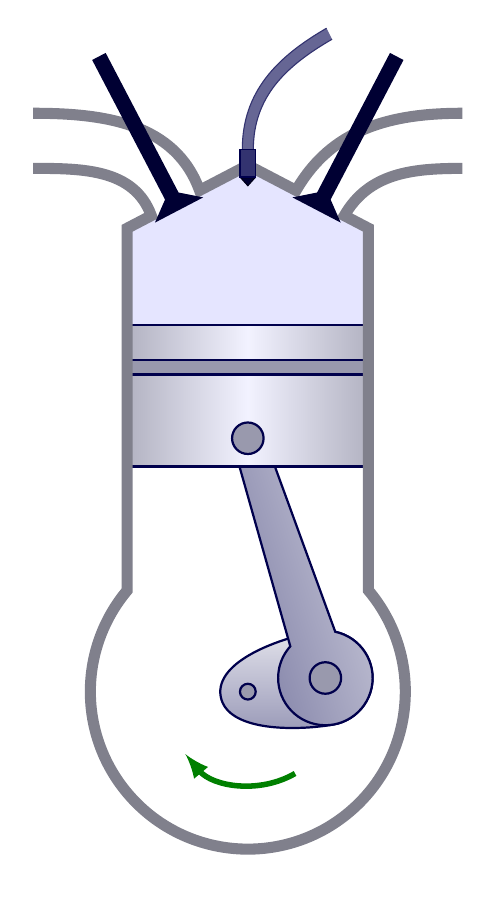
\begin{tikzpicture}
  \def\d{-60}
  \engine{10};
  \draw[vector] (\d:.6*\R) arc (\d:\d-80:.55*\R);
  %\draw[vector] (P) ++ (-.7,-.9) --++ (0,-1.1);
  \valveL{.1}
  \valveR{.1}
\end{tikzpicture}


% EXHAUST STROKE
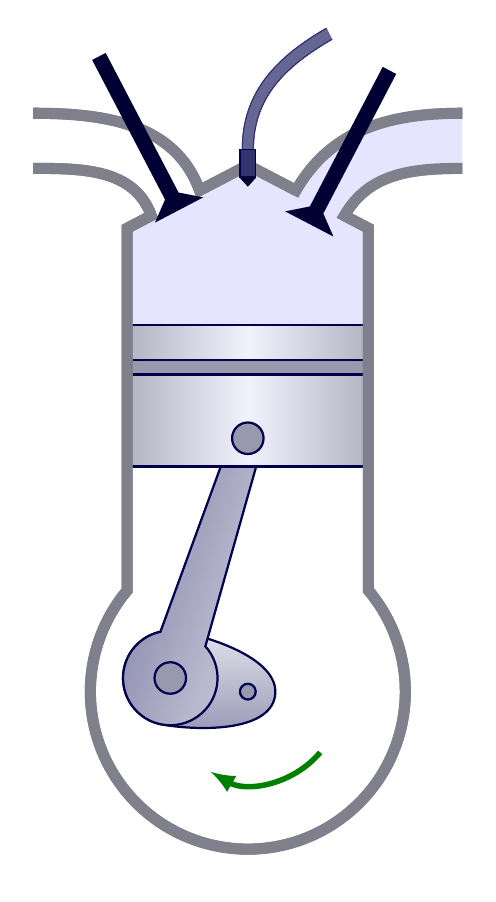
\begin{tikzpicture}
  \def\d{-40}
  \engine{-190};
  \draw[vector] (\d:.6*\R) arc (\d:\d-80:.55*\R);
  \fill[\gas]
    (VRo) to[out=60,in=-180] ++ (1.5,0.6) -- ($(VRo)+(1.5,1.3)$) to[out=180,in=60] (VRm) to[out=-270+\vr,in=-270+\vr] cycle;
  \wall
  \valveL{.1}
  \valveR{.3}
\end{tikzpicture}


\end{document}